\documentclass[tikz,border=7pt]{standalone}
\usepackage[T1]{fontenc}
\usetikzlibrary{arrows.meta,calc,positioning,shapes.geometric}
\begin{document}
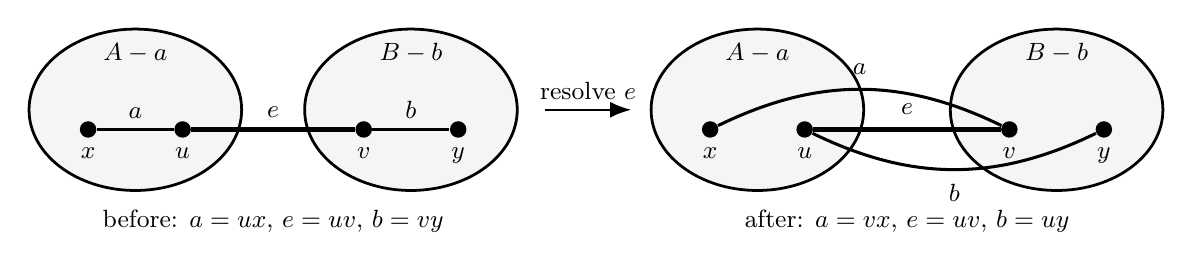
\begin{tikzpicture}[
  side/.style={ellipse,draw,line width=1pt,minimum width=2.7cm,
    minimum height=2.05cm,fill=black!4},
  vertex/.style={circle,fill=black,inner sep=2.1pt},
  edge/.style={line width=1.1pt},
  bridge/.style={line width=1.8pt},
  arrow/.style={-{Latex[length=2.7mm]},line width=.9pt},
  every node/.style={font=\small}
]
  % Before the move.
  \node[side] (A0) at (-5.25,0) {};
  \node[side] (B0) at (-1.75,0) {};
  \node at (-5.25,.72) {$A-a$};
  \node at (-1.75,.72) {$B-b$};
  \node[vertex,label=below:$x$] (x0) at (-5.85,-.25) {};
  \node[vertex,label=below:$u$] (u0) at (-4.65,-.25) {};
  \node[vertex,label=below:$v$] (v0) at (-2.35,-.25) {};
  \node[vertex,label=below:$y$] (y0) at (-1.15,-.25) {};
  \draw[edge] (x0)--(u0) node[midway,above] {$a$};
  \draw[bridge] (u0)--(v0) node[midway,above] {$e$};
  \draw[edge] (v0)--(y0) node[midway,above] {$b$};
  \node at (-3.5,-1.42) {before: $a=ux$, $e=uv$, $b=vy$};

  \draw[arrow] (-.05,0)--(1.05,0)
    node[midway,above] {resolve $e$};

  % After one resolution.
  \node[side] (A1) at (2.65,0) {};
  \node[side] (B1) at (6.45,0) {};
  \node at (2.65,.72) {$A-a$};
  \node at (6.45,.72) {$B-b$};
  \node[vertex,label=below:$x$] (x1) at (2.05,-.25) {};
  \node[vertex,label=below:$u$] (u1) at (3.25,-.25) {};
  \node[vertex,label=below:$v$] (v1) at (5.85,-.25) {};
  \node[vertex,label=below:$y$] (y1) at (7.05,-.25) {};
  \draw[bridge] (u1)--(v1) node[midway,above=.04cm] {$e$};
  \draw[edge] (x1) to[bend left=26]
    node[midway,above=.05cm] {$a$} (v1);
  \draw[edge] (u1) to[bend right=26]
    node[midway,below=.05cm] {$b$} (y1);
  \node at (4.55,-1.42) {after: $a=vx$, $e=uv$, $b=uy$};
\end{tikzpicture}
\end{document}
